\documentclass[conference]{IEEEtran}
\IEEEoverridecommandlockouts
\usepackage{cite}
\usepackage{amsmath,amssymb,amsfonts}
\usepackage{graphicx}
\usepackage{booktabs}
\usepackage{textcomp}
\usepackage{xcolor}
\usepackage[hidelinks]{hyperref}
\graphicspath{{figs/}}
\def\BibTeX{{\rm B\kern-.05em{\sc i\kern-.025em b}\kern-.08em
    T\kern-.1667em\lower.7ex\hbox{E}\kern-.125emX}}

\begin{document}

\title{Playback-Aware KV-Cache Management for Consistent Barge-In Handling\\in Cascaded Spoken Dialogue Systems}

% TODO: replace placeholder author block with real author information before submission.
\author{\IEEEauthorblockN{1\textsuperscript{st} Given Name Surname}
\IEEEauthorblockA{\textit{dept. name of organization} \\
\textit{name of organization}\\
City, Country \\
email address}
\and
\IEEEauthorblockN{2\textsuperscript{nd} Given Name Surname}
\IEEEauthorblockA{\textit{dept. name of organization} \\
\textit{name of organization}\\
City, Country \\
email address}
}

\maketitle

\begin{abstract}
Cascaded pipelines (streaming ASR $\rightarrow$ LLM $\rightarrow$ streaming TTS) remain the mainstream architecture for spoken dialogue systems, yet they suffer from a structural consistency flaw under user barge-in: the LLM's generation progress, the TTS synthesis progress, and the actual audio playback progress advance at different paces. If the system commits everything it has generated to the dialogue history, the model will later refer to content the user never heard. We formalize the generation--synthesis--playback progress pointers and the heard-boundary semantics, and build three mechanisms on top of them: (1) speculative generation scheduling that softens endpoint detection into an abortable process driven by continuous turn-detection confidence; (2) playback-aware KV-cache management that reverse-maps the playback position to a token boundary and performs explicit KV truncation with synchronized attention-mask and position-encoding correction plus chat-template role rebuilding; and (3) three policies for the interrupted history. On a 7B backbone with MultiWOZ-derived data, naive generation-point truncation lets unheard content resurface in up to 51\% of interrupted turns (surface-overlap criterion; 2.7\% under a conservative LLM-judge criterion), whereas our playback-aware truncation reduces the rate to zero by construction; the barge-in critical path is constantly sub-millisecond and independent of context length, with KV reuse up to 39.7$\times$ faster than re-prefilling at 8k context; speculative scheduling yields a continuously tunable waste--latency frontier, cutting post-utterance first-token latency from 48.5\,ms to 12.1\,ms for about 4.5\% token waste. To our knowledge this is the first open-source, reproducible cascaded implementation of playback-aware context management at the KV-cache level.
\end{abstract}

\begin{IEEEkeywords}
spoken dialogue system, barge-in, KV cache, speculative generation, context consistency, low latency
\end{IEEEkeywords}

\section{Introduction}
Large language models (LLMs) have moved voice assistants from command-style interaction toward natural conversation. In engineering practice, the cascaded architecture---streaming automatic speech recognition (ASR), an LLM, and streaming text-to-speech (TTS)---remains the mainstream design thanks to its modular controllability and strong reasoning ability. Beyond first-token latency, however, natural conversation requires graceful handling of \emph{barge-in}: users interrupt at any time, and whether the system can continue coherently depends on a subtle question---\emph{does what the system believes it said match what the user actually heard?}

In a cascade this mismatch is structural. The LLM generates tokens faster than the TTS synthesizes them, and synthesis in turn runs ahead of real-time playback. When the user interrupts mid-playback, a system that commits ``everything generated'' to the dialogue history will later refer to information the user never heard (``as I mentioned earlier\ldots''), derailing the conversation. Our experiments show that under such naive truncation, unheard-content references occur in up to 51\% of interrupted turns by a surface-overlap criterion (Sec.~\ref{sec:eval}).

The principle that \emph{dialogue history should equal what the user actually heard} is already practiced by commercial systems---OpenAI's Realtime API~\cite{openai_realtime}, Microsoft's Azure Voice Live~\cite{azure_voicelive}, and LiveKit Agents~\cite{livekit_agents}---and we explicitly do \emph{not} claim originality for the principle itself. These implementations, however, are closed-source or operate on managed transcript text; to our knowledge, no academic or open-source work realizes playback-aware context management \emph{inside} LLM inference via explicit KV-cache operations. This paper fills that gap. Our contributions are:
\begin{itemize}
  \item \textbf{Speculative generation scheduling.} Continuous turn-detection confidence with a speculation threshold turns endpoint detection into an abortable, roll-backable process; a nine-point waste--latency frontier on real data shows a knee where about 4.5\% token waste cuts post-utterance first-token latency from 48.5\,ms to 12.1\,ms (Sec.~\ref{sec:spec}, \ref{sec:eval}).
  \item \textbf{Playback-aware KV-cache management (core).} A four-way mapping timeline (token $\leftrightarrow$ segment $\leftrightarrow$ audio chunk $\leftrightarrow$ sample span), explicit truncation via \texttt{DynamicCache.crop} with synchronized mask/position handling, chat-template role-boundary rebuilding, and speculation rollback. The barge-in critical path is measured sub-millisecond, independent of context length; KV reuse is up to 39.7$\times$ faster than re-prefilling at 8k context (Sec.~\ref{sec:kv}, \ref{sec:eval}).
  \item \textbf{Interrupted-history policies.} Implementation and ablation of naive truncation, interruption marking, and lightweight-model rewriting (Sec.~\ref{sec:hist}, \ref{sec:eval}).
  \item \textbf{An open-source, reproducible reference implementation} with a dual-criterion consistency protocol including human arbitration.
\end{itemize}
The high-level idea of contribution 2 is prior art in commercial systems; our novelty lies in the open, reproducible, mechanism-level realization and its quantitative evaluation. The soft trigger and the rewriter use off-the-shelf models; we claim no model-level contribution.

\section{Related Work}
\subsubsection{Commercial practice} OpenAI's Realtime API provides \texttt{conversation.item.truncate}: on barge-in the client reports \texttt{audio\_end\_ms} and the server deletes unplayed audio and its transcript, explicitly ``so the context does not contain text the user has not heard''~\cite{openai_realtime}. Azure Voice Live offers \texttt{auto\_truncate}, updating the conversation context to the played portion~\cite{azure_voicelive}. LiveKit Agents commits only the actually-forwarded transcript and marks the message \texttt{interrupted}~\cite{livekit_agents}. Playback-aware truncation is thus established engineering practice; the differences to our work are open vs.\ closed source, explicit KV operations vs.\ transcript deletion, and measured playback vs.\ estimation---not whether the capability exists.

\subsubsection{Academic streaming dialogue} LTS-VoiceAgent~\cite{lts_voiceagent} reduces think-while-listening latency with semantic triggering and incremental reasoning, but does not address barge-in, playback position, or KV truncation. RelayS2S~\cite{relays2s} speculatively drafts a response prefix with a fast duplex model and verifies the handoff to a slower cascade; it shares our ``speculation for latency'' spirit but targets onset latency, not interrupt invalidation or KV management. Moshi~\cite{moshi} models both speakers as parallel streams in a frame-synchronous end-to-end architecture, so ``generation equals playback'' holds implicitly---which, from the opposite direction, confirms that the three-pointer mismatch is specific to cascades. FireRedChat~\cite{fireredchat} improves barge-in \emph{detection} with personalized streaming VAD but does not manage the half-spoken reply in the LLM context.

\subsubsection{KV-cache operations} The HuggingFace \texttt{DynamicCache} exposes a \texttt{crop} primitive~\cite{hf_kvcache}; serving frameworks optimize prefix caching for throughput. Orthogonal agent-side work prunes or discards KV state driven by text or tool logic---IntentKV~\cite{intentkv}, speculative tool calling~\cite{sia}---not by audio playback progress. We are not aware of a published open-source precedent that crops KV by playback position and rebuilds chat-template role boundaries in a speech cascade.

\section{Problem Formulation}\label{sec:form}
\subsection{Pipeline model and progress pointers}
Consider a cascade $\mathcal{S}=\langle \mathrm{ASR}, \mathrm{LLM}, \mathrm{CHK}, \mathrm{TTS}, \mathrm{PLY}\rangle$. Streaming ASR emits \emph{final} (non-revisable) text segments $u_1,u_2,\dots$, prefilling the LLM's KV cache $\mathcal{K}$ incrementally. The reply is generated autoregressively as tokens $y_1,\dots,y_G$; a sentence chunker CHK partitions the token stream into segments $f_j$ with contiguous token spans $[\mathrm{ts}(f_j),\mathrm{te}(f_j))$, the atomic unit of truncation. Streaming TTS renders each segment into audio chunks occupying sample span $[\mathrm{ss}(f_j),\mathrm{se}(f_j))$; the player reports the played-sample count $p$.

At any time $t$ three pointers measure progress on the same reply: generation $g(t)$ (tokens), synthesis $s(t)$ (segments), playback $p(t)$ (samples). Since generation outpaces synthesis and synthesis outpaces real-time playback,
\begin{equation}
p(t) \le s(t) \le g(t) \quad \forall t. \label{eq:invariant}
\end{equation}
Fig.~\ref{fig:pointers} illustrates the mismatch. Frame-synchronous end-to-end models such as Moshi collapse the three pointers into one; a cascade must manage the gap explicitly.

\begin{figure*}[t]
\centering

\includegraphics[width=0.92\textwidth]{fig3_1_en.pdf}
\caption{Three progress pointers and the heard boundary. At barge-in the playback pointer $p$ falls inside segment $f_3$; the heard boundary $H(p)=\mathrm{te}(f_3)$ rounds up at segment granularity, and $\varepsilon(p)$ is the bounded quantization error. Content between $p$ and $g$ is unheard; keeping it in history (B-gen) creates reference risk.}
\label{fig:pointers}
\end{figure*}

\subsection{Heard boundary and consistency}
Let barge-in occur with $p$ inside segment $f_k$ ($\mathrm{ss}(f_k)<p\le \mathrm{se}(f_k)$). The \emph{heard boundary} is
\begin{equation}
H(p)=\mathrm{te}(f_k), \label{eq:boundary}
\end{equation}
i.e., the interrupted segment is rounded up into ``heard.'' The history is \emph{user-perception consistent} iff the interrupted turn's assistant content is kept exactly on $[0,H(p))$. The naive alternative keeps all $G$ tokens, of which $y_{H(p)+1..G}$ are unheard. The \emph{quantization error} $\varepsilon(p)=H(p)-p^{\ast}$ (with $p^{\ast}$ the proportional token position of $p$ inside $f_k$) is bounded by one segment; we do not hide this error but quantify it with a \emph{strict} criterion below. Two truncation events share one mechanism: playback-time barge-in ($p>0$) and speculation invalidation ($p=0$, roll back to $H=0$).

\subsection{Reverse mapping and truncation legality}
The reverse map $\Phi: p \rightarrow f_k \rightarrow [\mathrm{ts}(f_k),\mathrm{te}(f_k)) \rightarrow H(p)$ must resolve in near-constant time---it sits on the ``stop-on-interrupt'' critical path. Truncating $\mathcal{K}$ to absolute position $N=a_0+H(p)$ (with $a_0$ the assistant-turn start) is \emph{legal} iff (i) KV tensors, attention mask, and recorded sequence length agree at $N$; (ii) subsequent position encodings continue from $N$; (iii) chat-template role boundaries are rebuilt so later turns remain structurally valid. Conditions (ii) and (iii) are the main engineering pitfalls; all three are runtime-checked throughout our experiments.

\subsection{Metrics}
\emph{Latency:} $\mathrm{TTFT}_{\mathrm{eff}}$ measures true-end-of-speech to first usable token (user-perceived; surviving speculation makes it $\approx 0$); mouth-to-ear is modeled as first-segment-ready plus the TTS first-chunk latency from a measured device profile. \emph{Consistency:} the unheard-content reference rate under a \emph{loose} criterion (complete unheard segments; zero under our method \emph{by construction}---the experiment quantifies the baseline's failure rate, not ours) and a \emph{strict} criterion (adds the unplayed tail of the partial segment, i.e., the consequence of $\varepsilon$). Reference detection uses two instruments whose agreement we report: a lexical rule detector (systematically high; upper bound) and an LLM judge for specific-information reference (conservative; lower bound), plus human arbitration on a stratified sample. \emph{Efficiency:} the speculation waste rate
\begin{equation}
\rho=\frac{\sum \text{invalidated speculative tokens}}{\sum \text{invalidated speculative tokens}+\sum \text{final tokens}}, \label{eq:rho}
\end{equation}
and the $(\rho,\mathrm{TTFT}_{\mathrm{eff}})$ frontier under threshold sweep.

\section{System Design}\label{sec:design}
Fig.~\ref{fig:arch} shows the overall architecture: the phase-one streaming-ASR + incremental-prefill pipeline is extended with an output-side three-stage pipeline (chunking $\rightarrow$ streaming TTS $\rightarrow$ playback) and two control mechanisms. Design principles: (P1) \emph{history = what the user heard} (the principle itself is prior art; we contribute its explicit KV-level realization on an open cascade); (P2) \emph{trade redundant, measurable computation for interaction fluency}.

\begin{figure*}[t]
\centering
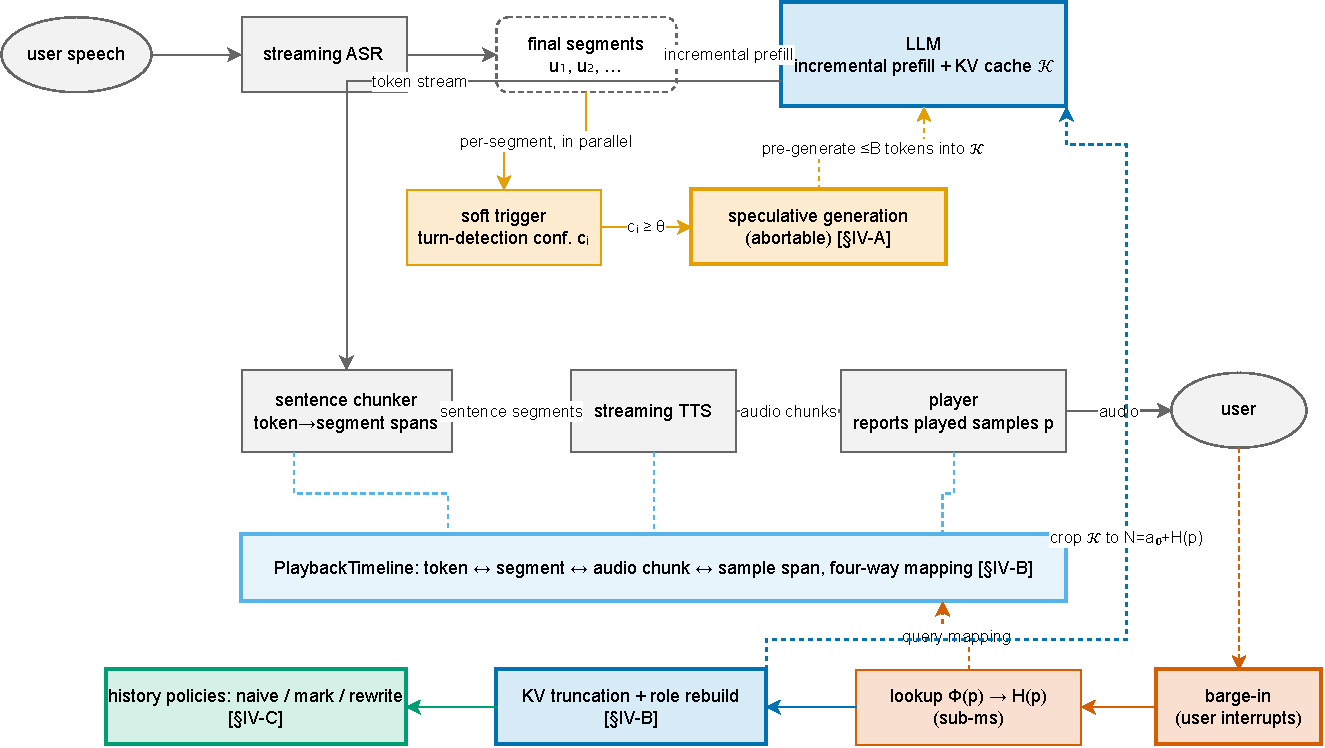
\includegraphics[width=0.9\textwidth]{fig4_1_en.pdf}
\caption{System architecture. Top: input pipeline and soft-trigger-driven speculative generation (Sec.~\ref{sec:spec}). Middle: output pipeline and the four-way mapping timeline. Bottom: barge-in chain---lookup $\Phi(p)\!\rightarrow\!H(p)$, KV truncation + role rebuild (Sec.~\ref{sec:kv}), history policies (Sec.~\ref{sec:hist}).}
\label{fig:arch}
\end{figure*}

\subsection{Speculative Generation Scheduling}\label{sec:spec}
An off-the-shelf turn-detection model (TEN~\cite{ten_turn}) yields a continuous confidence $c_i$ for the accumulated user text. When $c_i\ge\theta$ the system records the speculation start $b:=|\mathcal{K}|$, injects the assistant role marker, and pre-generates up to $B$ tokens (the speculation budget bounds single-shot invalidation cost). If another user segment arrives, the speculation is invalidated: KV is cropped back to $b$ (a degenerate case of playback truncation with $p=0$) and the output counts toward $\rho$. If the user has truly finished and a speculation survives, cached tokens are emitted immediately ($\mathrm{TTFT}_{\mathrm{eff}}\approx0$) and generation continues. The trigger runs on the text side in parallel with the segment's KV prefill, adding no end-to-end latency. Sweeping $\theta$ turns the endpoint decision into a tunable knob along the $(\rho,\mathrm{TTFT}_{\mathrm{eff}})$ frontier.

\subsection{Playback-Aware KV-Cache Management}\label{sec:kv}
\subsubsection{Four-way mapping timeline} An append-only structure keyed by segment records $\langle f_j, [\mathrm{ts},\mathrm{te}), \text{chunk list}, [\mathrm{ss},\mathrm{se}), \text{state}\rangle$ with states speculative $\rightarrow$ synthesizing $\rightarrow$ enqueued $\rightarrow$ playing $\rightarrow$ played/invalidated. Three producers write their own dimensions (generation thread: token$\leftrightarrow$segment; TTS thread: segment$\leftrightarrow$chunks and the sample axis; player thread: atomic update of $p$). Since segments per turn are few, one table lock plus a lock-free playback cursor meets the sub-millisecond lookup requirement. Token spans come from whitespace-insensitive character-count alignment between the chunker's text and the decoded token stream, verified lossless.

\subsubsection{Legal truncation} On barge-in, $\Phi(p)$ yields $H(p)$ and the cache is cropped to $N$: KV tensor slicing (\texttt{DynamicCache.crop}~\cite{hf_kvcache}), \emph{synchronized} attention-mask shortening to $N$ (the mask length is the source of truth for subsequent past length---cropping KV without the mask silently corrupts position encoding), and ledger updates so later prefills recompute positions explicitly from $N$. The critical path is exactly this tensor slicing: sub-millisecond.

\subsubsection{Role-boundary rebuild} KV is a flat sequence; role structure exists only in chat-template markers. We derive the role-switch string (e.g., ChatML \texttt{<|im\_end|>}\ldots\texttt{<|im\_start|>user}) from the tokenizer's template by differencing, and prefill it as ordinary text through the same explicit mask/position path---no special kernel. This rebuild (tens of ms) is \emph{off} the critical path: stopping playback plus truncation suffices for the perceived ``instant stop,'' and the rebuild is deferred until the next user input. The generation loop writes each new token's KV, mask, and id back into a single accumulating cache, making assistant-side KV first-class, truncatable state across multiple turns.

\subsection{Interrupted-History Policies}\label{sec:hist}
With playback truncation the history may end mid-sentence. We compare, on top of it: \emph{naive} (leave as-is); \emph{mark} (append an interruption marker, zero cost); \emph{rewrite} (only for partial cuts, a 0.6B model rewrites the half sentence into a natural ending, constrained to add no information; the KV of the interrupted assistant span is recomputed from the rewritten text, and rewriting runs concurrently with the user's interrupting speech).

\section{Evaluation}\label{sec:eval}
\subsection{Setup}
Two RTX 3090 GPUs; main LLM Qwen2-7B-Instruct~\cite{qwen2}; soft trigger TEN Turn Detection (7.6B, text-side; calibrated pairwise AUC $=1.00$ on our utterances)~\cite{ten_turn}; rewriter Qwen3-0.6B~\cite{qwen3}; LLM judge Mistral-7B-Instruct-v0.3~\cite{mistral7b} (a different model family from the backbone, to avoid same-family bias); streaming TTS CosyVoice2-0.5B~\cite{cosyvoice2} with a measured timing profile (3175 samples per non-space character at 24\,kHz; first-chunk latency 2433.6\,ms on 3090 without TensorRT; RTF 0.513). Data derive from MultiWOZ~2.1~\cite{multiwoz21} (fixed seed): 103 multi-turn dialogues and 100 clause-split utterances, English. Barge-in is injected deterministically at playback fractions 25\%/50\%/75\% and at clean segment boundaries (control), with the playback pointer as ground truth---fully reproducible. Conditions: System~A (non-streaming baseline: full prefill after end of speech, full generation, whole-utterance synthesis), B-ours (playback truncation), B-gen (generation truncation, keeping all generated content). Synthesis-point truncation is equivalent to B-gen under our synchronous-synthesis mock and is not claimed as validated.

\subsection{Consistency (main result)}
Table~\ref{tab:consistency} reports the unheard-content reference rate ($n{=}412$ per condition). Under the loose criterion B-ours is zero \emph{by construction} (the mechanism leaves no unheard segment in history)---the measured quantity is the baseline's failure rate: 51.0\% of B-gen's follow-up replies reuse unheard surface content, and even the most conservative judge criterion leaves 2.7\% of turns where the model ``quotes what it never said'' ($p<10^{-3}$, Fisher exact). The rate grows the earlier the interruption (85.4\% at 25\% playback vs.\ 20.4\% at 75\%, rule criterion; Fig.~\ref{fig:positions}). Under the strict criterion the residual tail of partial segments makes the rule detector report 51.0\% for B-ours---but this is a lexical-overlap upper bound; the judge reports 2.4\%, statistically indistinguishable from B-gen's 2.9\% ($p{=}0.83$): segment-granularity truncation carries no measurable extra cost in the specific-reference sense. Clean-boundary injections show 103/103 zero strict residue, a data-level check of the boundary semantics.

The two instruments disagree strongly on real data (Cohen's $\kappa\approx0.05$): MultiWOZ domain words (hotel, book, train) make the rule detector over-trigger. We therefore read the rule criterion as an upper bound and the judge as a lower bound, and arbitrate with 37 human-annotated samples: human--judge agreement is moderate-to-strong ($84.6\%$, $\kappa=0.649$) while human--rule agreement is no better than chance ($\kappa=-0.073$), supporting the judge as the headline instrument. Notably, humans judged 0/24 strict-criterion samples to be actual specific references, empirically vindicating segment-level truncation granularity.

\begin{table}[t]
\caption{Unheard-content reference rate (E3, $n{=}412$ per condition)}
\label{tab:consistency}
\centering
\begin{tabular}{llccc}
\toprule
Criterion & Detector & B-ours & B-gen & $p$ \\
\midrule
loose & rule & \textbf{0.0\%} (by constr.) & 51.0\% & $1.8{\times}10^{-79}$ \\
strict & rule & 51.0\% & 73.3\% & $5.0{\times}10^{-11}$ \\
loose & judge & \textbf{0.0\%} & 2.7\% & $9.1{\times}10^{-4}$ \\
strict & judge & 2.4\% & 2.9\% & 0.83 (n.s.) \\
\bottomrule
\end{tabular}
\end{table}

\begin{figure}[t]
\centering
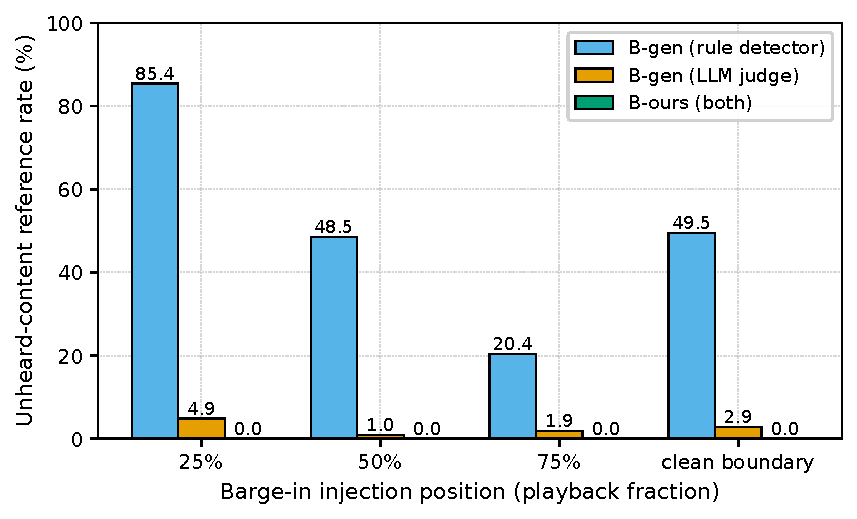
\includegraphics[width=\linewidth]{fig6_1_en.pdf}
\caption{Unheard-content reference rate by injection position. B-gen decreases monotonically with later interruption; B-ours is zero under both criteria---a constructive guarantee of the mechanism, not a statistical finding.}
\label{fig:positions}
\end{figure}

\subsection{Waste--latency frontier}
Fig.~\ref{fig:frontier} shows the nine-point sweep of $\theta$ ($n{=}100$ per point) including the never-speculate sentinel. The frontier is monotone with a clear knee ($\theta\in[0.85,0.97]$): at $\theta{=}0.92$, 4.5\% waste buys $\mathrm{TTFT}_{\mathrm{eff}}$ 48.5$\rightarrow$12.1\,ms ($-75\%$); at $\theta{=}0.9688$, 0.8\% waste still yields $-40\%$. At the aggressive end ($\theta\le0.4$) waste is 14--29\% while $\mathrm{TTFT}_{\mathrm{eff}}\approx0$: speculation is almost always ready before the user finishes. Note the 7B ``never speculate'' full TTFT is only 48.5\,ms thanks to streaming prefill, so the \emph{relative} gains (75--99\%) generalize better than the absolute milliseconds; for larger models or longer reply prefixes the absolute gain scales up.

\begin{figure}[t]
\centering
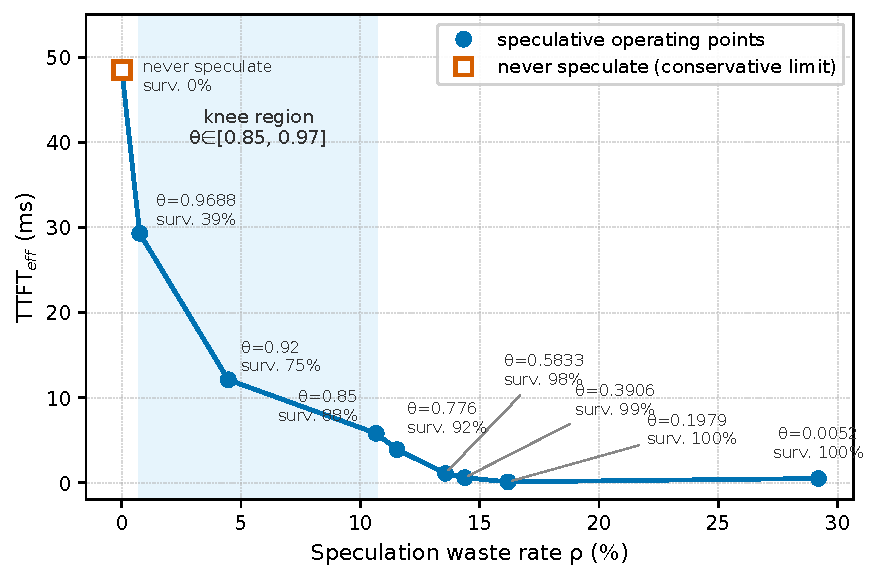
\includegraphics[width=\linewidth]{fig6_2_en.pdf}
\caption{Speculation waste rate vs.\ $\mathrm{TTFT}_{\mathrm{eff}}$: a continuously tunable frontier; the open square is the never-speculate conservative limit.}
\label{fig:frontier}
\end{figure}

\subsection{End-to-end latency}
At the $\theta{=}0.391$ operating point ($n{=}100$), measured $\mathrm{TTFT}$: System~A 27.4\,ms vs.\ B-ours $\mathrm{TTFT}_{\mathrm{eff}}$ \textbf{0.6\,ms} (97.9\% reduction). Modeled mouth-to-ear (first-segment ready + TTS first chunk, 3090 profile): A 9080\,ms (must finish generating, then synthesize the whole reply) vs.\ B-ours 2482\,ms, of which 2434\,ms is TTS first-chunk latency. This term is strongly deployment-dependent: extrapolating with the vendor-reported A100+TensorRT first-chunk figure ($\approx$45\,ms) brings B-ours to the $\sim$100\,ms range, whereas System~A's wait-for-everything cost is structural and grows with reply length.

\subsection{KV reuse vs.\ re-prefill}
Fig.~\ref{fig:kvreuse} sweeps context length 275--8192 tokens (median of 5, 7B). The critical path (lookup + crop) is 0.31--0.34\,ms, constant in context length; role rebuild (25--47\,ms) is off the critical path; re-prefilling the heard-boundary context grows linearly, reaching 1.86\,s at 8k---a 39.7$\times$ gap that widens as multi-turn context grows.

\begin{figure}[t]
\centering

\includegraphics[width=\linewidth]{fig6_4_en.pdf}
\caption{Barge-in response paths vs.\ re-prefill across context lengths (log--log). Lookup+crop is sub-ms and length-independent; re-prefill grows nearly linearly (39.7$\times$ at 8k).}
\label{fig:kvreuse}
\end{figure}

\subsection{Interrupted-history policies (honest null)}
Judge coherence (1--5, $n{=}100$ per policy): naive 3.76, rewrite 3.62, mark 3.29; rewriting is \emph{not} better than naive truncation (Wilcoxon $p{=}0.32$). Plausible reasons: the 7B backbone is already robust to half-sentence history; the 0.6B rewriter's paraphrasing dilutes contextual cues. The engineering claims still hold---rewrite latency mean 639\,ms, P90 937\,ms, hideable inside the user's interrupting speech---so we position rewriting as an exploratory mechanism pending stronger rewriters and pairwise-preference evaluation.

\section{Discussion and Limitations}
\emph{Relation to commercial systems.} The differences are operation level (explicit KV truncation preserving cross-turn KV reuse vs.\ transcript deletion), position source (player-reported sample counts and reverse mapping vs.\ real-time-rate assumptions or client-reported offsets), and inspectability (all mappings and decisions logged; experiments reproducible). None of these support a claim that commercial systems lack the capability. \emph{Instrumentation.} The rule detector over-triggers on domain words; our upper-bound/lower-bound/arbitration protocol mitigates but a larger human study would tighten the interval. \emph{Timing model.} Mouth-to-ear is modeled from a measured profile; first-chunk latency varies by two orders of magnitude across inference stacks, so cross-system comparisons need care. \emph{Scope.} Experiments cover English task-oriented dialogues with deterministic injected barge-in; open-domain speech, natural interruption behavior, and Chinese-language paths are future work. The mechanisms themselves bind to no specific stack: any sentence-level streaming TTS, any causal LM in the \texttt{DynamicCache} ecosystem, and any confidence-emitting endpoint model can be substituted.

\section{Conclusion}
We formalized the generation--synthesis--playback mismatch that makes cascaded voice agents misremember what they said, and presented an open, reproducible cascade in which dialogue history provably equals what the user heard: speculative scheduling makes endpoint detection a tunable waste--latency knob (48.5$\rightarrow$12.1\,ms at 4.5\% waste); playback-aware KV truncation answers barge-in in sub-millisecond time independent of context length (39.7$\times$ over re-prefill at 8k); and a dual-criterion protocol with human arbitration shows naive truncation resurfaces unheard content in 51\%/2.7\% (surface/specific) of interrupted turns while our mechanism eliminates it by construction, with no measurable cost from segment-granularity truncation. Code, data derivations, and per-turn instrumentation are open-sourced for reproduction.

\section*{Acknowledgment}
% TODO: add funding / acknowledgment before submission.
Large language models were used to assist with literature retrieval verification, figure scripting, and language polishing of this manuscript; all technical content, experiments, and conclusions were produced and verified by the authors.

\bibliographystyle{IEEEtran}
\bibliography{references}

\end{document}
